\subsubsection{Каскад ОБ}

Принципиальная схема:
\begin{center}
	\begin{figure}[h!]
		\center{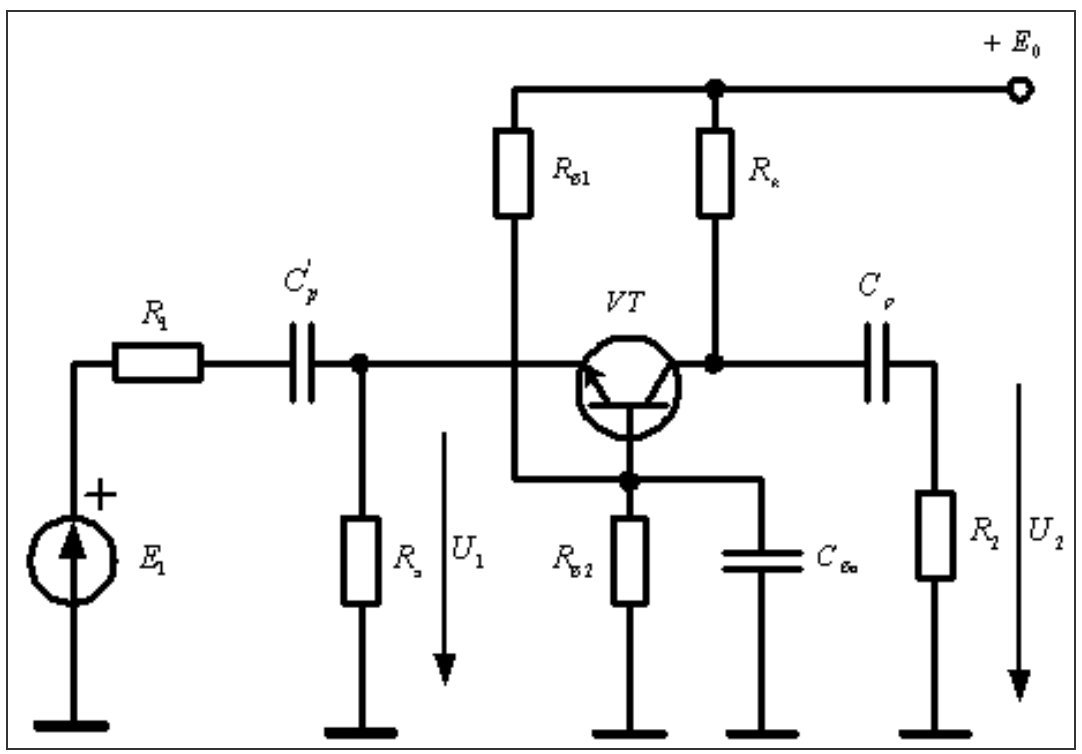
\includegraphics[scale=0.2]{ob.png}}
		\caption{каскад с ОБ}
	\end{figure}
\end{center}
Эквивалентная схема:
\begin{center}
	\begin{figure}[h!]
		\center{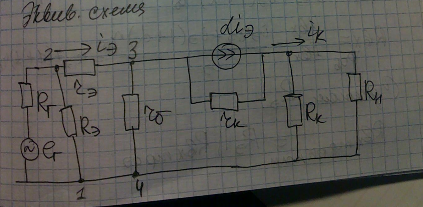
\includegraphics[scale=0.9]{eob.png}}
		\caption{эквивалентная схема с ОБ}
	\end{figure}
\end{center}

1.Входное сопротивление:
$$R_\textit{вх}=\frac{U_\textit{вх}}{i_\textit{вх}}$$

$$U_\textit{вх}=E_\textit{г}-i_\textit{вх}R_\textit{г}$$

1)Без учета $R_\textit{э}$, тогда $i_\textit{вх}=i_\textit{э}$

$U_\textit{вх}=\varphi_2-\varphi_1=i_\textit{э}r_\textit{э}+i_\textit{б}r_\textit{б}$
(контур 1 по II-му закону Кирхгофа)
Из эквивалентной схемы:
$i_\textit{б}=(\alpha+1)i_\textit{э}$ - По первому з-ну Кирхгофа

$U_\textit{вх}=i_\textit{э}r_\textit{э}+(\alpha+1)i_\textit{э}r\textit{б}$

$R_\textit{вхтроб}=\frac{U_\textit{вх}}{i_\textit{вх}}=\frac{i_\textit{э}r_\textit{э}+(\alpha+1)i_\textit{э}r_\textit{э}}{i_\textit{э}}$

$$
R_\textit{вхтроб}=r_\textit{э} + (\alpha+1)r_\textit{б}
$$

2)C учетом $R_\textit{э}$ получаем

$$
R_\textit{вхтроб}=R_\textit{э}||R_\textit{вхтроэ}
$$

2. Выходное сопротивление:
 Выходное сопротивление определяется при отключении нагрущки и при нулевом входном сигнале
 
 $$R_\textit{вых}=\frac{U_\textit{хх}}{i_\textit{кз}}$$

$ I_\textit{кз}\approx \alpha i_\textit{э}$

$$
\frac{I_\textit{к}}{I_\textit{э}}=\alpha,\Rightarrow R_\textit{вых}=\frac{I_\textit{к}R_\textit{к}}{\alpha I_\textit{э}}=\frac{\alpha I_\textit{э}R_\textit{к}}{\alpha I_\textit{э}}\approx R_\textit{к}
$$

3. Коэффициент передачи по напряжению:

$$
K_\textit{uоб}=\frac{U_\textit{вых}}{U_\textit{вх}}=\frac{\alpha(R_\textit{к}||R_\textit{н})}{R_\textit{вхтроб}}=\frac{B(R_\textit{k}||R_\textit{н})}{R_\textit{вхтроэ}}
$$

4. Коэффициент передачи по току:

$$K_\textit{iоэ}=\frac{i_\textit{вых}}{i_\textit{вх}}=\frac{i_\textit{н}}{i_\textit{вх}}$$

$i_H=i_K\frac{R_k}{R_H+R_k}$

$i_{R_\textit{э}}=i_\textit{э}\frac{R_\textit{вхтроб}}{R_\textit{Э}}$

$$
K_{I_\textit{ОБ}}=i_k\frac{R_k}{R_k+R_H}\frac{1}{\frac{R_\textit{вхтроб}+R_\textit{э}}{R_\textit{э}}i_\textit{э}}=\alpha \frac{R_k}{R_k+R_H} \frac{R_\textit{э}}{R_\textit{вхтроб}+R_\textit{э}}
$$

\pagebreak
